\documentclass{article}

% chinese fonts
\usepackage{ctex}

% math fonts
\usepackage{amsmath}
\usepackage{amsthm}
\usepackage{amssymb}
\usepackage{bm}

% figures
\usepackage{tikz}
\usepackage{graphicx}
\graphicspath{{./figures/}}

% tables
\usepackage{tabularx}
\usepackage{booktabs}
\usepackage{multirow}

% codes
\usepackage{listings}
\lstset{language     = Matlab,
        basicstyle   = \ttfamily,
        keywordstyle = \color{cyan},
        rulecolor    = \color{black},
        commentstyle = \color{green},
        keepspaces   = true,
        tabsize      = 4,
}

% hyperlinks
\usepackage{hyperref}
\hypersetup{
  breaklinks,
  colorlinks = true,
  citecolor  = blue,
  linkcolor  = red,
  urlcolor   = magenta,
}

% algorithms
\usepackage{algorithm}
\usepackage{algorithmic}

% bibliography
\usepackage[sort&compress,numbers]{natbib}

% About:  Macros for Vector, Matrix, Tensor, Math Operator and Misc
% Author: Jingxuan Yang

% vectors
\newcommand{\va}{\bm{a}}       \newcommand{\vah}{\hat{\bm{a}}}        \newcommand{\ah}{\hat{a}}    \newcommand{\vat}{\tilde{\bm{a}}}       \newcommand{\at}{\tilde{a}}
\newcommand{\vb}{\bm{b}}       \newcommand{\vbh}{\hat{\bm{b}}}        \newcommand{\bh}{\hat{b}}    \newcommand{\vbt}{\tilde{\bm{b}}}       \newcommand{\bt}{\tilde{b}}
\newcommand{\vc}{\bm{c}}       \newcommand{\vch}{\hat{\bm{c}}}        \newcommand{\ch}{\hat{c}}    \newcommand{\vct}{\tilde{\bm{c}}}       \newcommand{\ct}{\tilde{c}}
\newcommand{\vd}{\bm{d}}       \newcommand{\vdh}{\hat{\bm{d}}}        \newcommand{\dhat}{\hat{d}}  \newcommand{\vdt}{\tilde{\bm{d}}}       \newcommand{\dt}{\tilde{d}}
\newcommand{\ve}{\bm{e}}       \newcommand{\veh}{\hat{\bm{e}}}        \newcommand{\eh}{\hat{e}}    \newcommand{\vet}{\tilde{\bm{e}}}       \newcommand{\et}{\tilde{e}}
\newcommand{\vf}{\bm{f}}       \newcommand{\vfh}{\hat{\bm{f}}}        \newcommand{\fh}{\hat{f}}    \newcommand{\vft}{\tilde{\bm{f}}}       \newcommand{\ft}{\tilde{f}}
\newcommand{\vg}{\bm{g}}       \newcommand{\vgh}{\hat{\bm{g}}}        \newcommand{\gh}{\hat{g}}    \newcommand{\vgt}{\tilde{\bm{g}}}       \newcommand{\gt}{\tilde{g}}
\newcommand{\vh}{\bm{h}}     \newcommand{\vhh}{\hat{\bm{h}}}        \newcommand{\hh}{\hat{h}}    \newcommand{\vht}{\tilde{\bm{h}}}       \newcommand{\htild}{\tilde{h}}
\newcommand{\vi}{\bm{i}}       \newcommand{\vih}{\hat{\bm{i}}}        \newcommand{\ih}{\hat{i}}    \newcommand{\vit}{\tilde{\bm{i}}}       \newcommand{\itild}{\tilde{i}}
\newcommand{\vj}{\bm{j}}       \newcommand{\vjh}{\hat{\bm{j}}}        \newcommand{\jh}{\hat{j}}    \newcommand{\vjt}{\tilde{\bm{j}}}       \newcommand{\jt}{\tilde{j}}
\newcommand{\vk}{\bm{k}}       \newcommand{\vkh}{\hat{\bm{k}}}        \newcommand{\kh}{\hat{k}}    \newcommand{\vkt}{\tilde{\bm{k}}}       \newcommand{\kt}{\tilde{k}}
\newcommand{\vl}{\bm{l}}       \newcommand{\vlh}{\hat{\bm{l}}}        \newcommand{\lh}{\hat{l}}    \newcommand{\vlt}{\tilde{\bm{l}}}       \newcommand{\lt}{\tilde{l}}
\newcommand{\vm}{\bm{m}}       \newcommand{\vmh}{\hat{\bm{m}}}        \newcommand{\mh}{\hat{m}}    \newcommand{\vmt}{\tilde{\bm{m}}}       \newcommand{\mt}{\tilde{m}}
\newcommand{\vn}{\bm{n}}       \newcommand{\vnh}{\hat{\bm{n}}}        \newcommand{\nh}{\hat{n}}    \newcommand{\vnt}{\tilde{\bm{n}}}       \newcommand{\nt}{\tilde{n}}
\newcommand{\vo}{\bm{o}}       \newcommand{\voh}{\hat{\bm{o}}}        \newcommand{\oh}{\hat{o}}    \newcommand{\vot}{\tilde{\bm{o}}}       \newcommand{\ot}{\tilde{o}}
\newcommand{\vp}{\bm{p}}       \newcommand{\vph}{\hat{\bm{p}}}        \newcommand{\ph}{\hat{p}}    \newcommand{\vpt}{\tilde{\bm{p}}}       \newcommand{\pt}{\tilde{p}}
\newcommand{\vq}{\bm{q}}       \newcommand{\vqh}{\hat{\bm{q}}}        \newcommand{\qh}{\hat{q}}    \newcommand{\vqt}{\tilde{\bm{q}}}       \newcommand{\qt}{\tilde{q}}
\newcommand{\vr}{\bm{r}}       \newcommand{\vrh}{\hat{\bm{r}}}        \newcommand{\rh}{\hat{r}}    \newcommand{\vrt}{\tilde{\bm{r}}}       \newcommand{\rt}{\tilde{r}}
\newcommand{\vs}{\bm{s}}       \newcommand{\vsh}{\hat{\bm{s}}}        \newcommand{\sh}{\hat{s}}    \newcommand{\vst}{\tilde{\bm{s}}}       \newcommand{\st}{\tilde{s}}
\newcommand{\vt}{\bm{t}}       \newcommand{\vth}{\hat{\bm{t}}}        \newcommand{\that}{\hat{t}}  \newcommand{\vtt}{\tilde{\bm{t}}}       \newcommand{\ttil}{\tilde{t}}
\newcommand{\vu}{\bm{u}}       \newcommand{\vuh}{\hat{\bm{u}}}        \newcommand{\uh}{\hat{u}}    \newcommand{\vut}{\tilde{\bm{u}}}       \newcommand{\ut}{\tilde{u}}
\newcommand{\vv}{\bm{v}}       \newcommand{\vvh}{\hat{\bm{v}}}        \newcommand{\vhat}{\hat{v}}    \newcommand{\vvt}{\tilde{\bm{v}}}       \newcommand{\vtild}{\tilde{v}}
\newcommand{\vw}{\bm{w}}       \newcommand{\vwh}{\hat{\bm{w}}}        \newcommand{\wh}{\hat{w}}    \newcommand{\vwt}{\tilde{\bm{w}}}       \newcommand{\wt}{\tilde{w}}
\newcommand{\vx}{\bm{x}}       \newcommand{\vxh}{\hat{\bm{x}}}        \newcommand{\xh}{\hat{x}}    \newcommand{\vxt}{\tilde{\bm{x}}}       \newcommand{\xt}{\tilde{x}}
\newcommand{\vy}{\bm{y}}       \newcommand{\vyh}{\hat{\bm{y}}}        \newcommand{\yh}{\hat{y}}    \newcommand{\vyt}{\tilde{\bm{y}}}       \newcommand{\yt}{\tilde{y}}
\newcommand{\vz}{\bm{z}}       \newcommand{\vzh}{\hat{\bm{z}}}        \newcommand{\zh}{\hat{z}}    \newcommand{\vzt}{\tilde{\bm{z}}}       \newcommand{\zt}{\tilde{z}}

\newcommand{\valpha}{\bm{\alpha}}
\newcommand{\vbeta}{\bm{\beta}}
\newcommand{\vgamma}{\bm{\gamma}}
\newcommand{\vtheta}{\bm{\theta}}
\newcommand{\vlambda}{\bm{\lambda}}
\newcommand{\vmu}{\bm{\mu}}
\newcommand{\vomega}{\bm{\omega}}

\newcommand{\mSigma}{\bm{\Sigma}}

\newcommand{\Fc}{\mathcal{F}}
\newcommand{\Xc}{\mathcal{X}}
\newcommand{\Yc}{\mathcal{Y}}
\newcommand{\Zc}{\mathcal{Z}}
\newcommand{\Gc}{\mathcal{G}}
\newcommand{\Hc}{\mathcal{H}}
\newcommand{\Dc}{\mathcal{D}}
\newcommand{\Cc}{\mathcal{C}}
\newcommand{\Rc}{\mathcal{R}}

% matrices
\newcommand{\ma}{\bm{A}}
\newcommand{\mb}{\bm{B}}
\newcommand{\md}{\bm{D}}
\newcommand{\mH}{\bm{H}}
\newcommand{\mE}{\bm{E}}
\newcommand{\mi}{\bm{I}}
\newcommand{\mk}{\bm{K}}
\newcommand{\ml}{\bm{L}}
\newcommand{\mn}{\bm{N}}
\newcommand{\mP}{\bm{P}}
\newcommand{\mq}{\bm{Q}}
\newcommand{\mr}{\bm{R}}
\newcommand{\mU}{\bm{u}}
\newcommand{\mv}{\bm{v}}
\newcommand{\mw}{\bm{W}}
\newcommand{\mx}{\bm{X}}
\newcommand{\my}{\bm{Y}}
\newcommand{\mz}{\bm{Z}}

% tensors
\newcommand{\tp}{\mathsf{P}}
\newcommand{\tu}{\mathsf{U}}
\newcommand{\tx}{\mathsf{X}}
\newcommand{\ty}{\mathsf{Y}}
\newcommand{\tz}{\mathsf{Z}}
\newcommand{\tw}{\mathsf{W}}
\newcommand{\tf}{\mathsf{F}}
\newcommand{\ta}{\mathsf{A}}
\renewcommand{\th}{\mathsf{H}}

% norms
\newcommand{\mynorm}[2]{\| {#1} \|_{#2}}
\newcommand{\norm}[2]{\mynorm{#1}{#2}}
\newcommand{\bignorm}[2]{\left\| {#1} \right\|_{#2}}
\newcommand{\norml}[1]{\mynorm{#1}{1}}
\newcommand{\bignorml}[1]{\bignorm{#1}{1}}
\newcommand{\infnorm}[1]{\mynorm{#1}{\infty}}
\newcommand{\biginfnorm}[1]{\bignorm{#1}{\infty}}
\newcommand{\oneinf}{\ell_{1,\infty}}
\newcommand{\onetwo}{\ell_{1,2}}
\newcommand{\oneinfnorm}[1]{\mynorm{#1}{1,\infty}}
\newcommand{\bigoneinf}[1]{\bignorm{#1}{1,\infty}}
\newcommand{\onetwonorm}[1]{\mynorm{#1}{1,2}}
\newcommand{\bigonetwo}[1]{\bignorm{#1}{1,2}}
\newcommand{\enorm}[1]{\mynorm{#1}{2}}
\newcommand{\bigenorm}[1]{\bignorm{#1}{2}}
\newcommand{\znorm}[1]{\mynorm{#1}{0}}
\newcommand{\bigznorm}[1]{\bignorm{#1}{0}}
\newcommand{\frob}[1]{\|{#1}\|_{\text{F}}}
\newcommand{\bigfrob}[1]{\bignorm{#1}{\text{F}}}
\newcommand{\grpnorm}[2]{\norm{#1}{\text{Gr}(#2)}}

% math operators
\DeclareMathOperator*{\argmin}{argmin}
\DeclareMathOperator*{\argmax}{argmax}
\DeclareMathOperator{\divg}{div}
\DeclareMathOperator{\dom}{dom}
\DeclareMathOperator{\interior}{int}
\DeclareMathOperator{\ri}{ri}
\DeclareMathOperator{\sgn}{sgn}
\DeclareMathOperator{\trace}{Tr}
\DeclareMathOperator{\diag}{diag}
\DeclareMathOperator{\rank}{rank}
\DeclareMathOperator{\range}{range}
\DeclareMathOperator{\vect}{vec}
\DeclareMathOperator{\prox}{prox}
\DeclareMathOperator{\intr}{int}
\DeclareMathOperator{\relint}{ri}

% misc
\newcommand{\gs}{\geqslant}
\newcommand{\ls}{\leqslant}
\newcommand{\set}[1]{\left\{ {#1}\right\}}

\newcommand{\defeq}{\ \stackrel{\text{def}}{=}\ }
\newcommand{\ip}[2]{\left\langle#1, #2\right\rangle}
\newcommand{\reals}{\mathbb{R}}
\newcommand{\complex}{\mathbb{C}}
\newcommand{\half}{\frac{1}{2}}

\newtheorem{theorem}{Theorem}
\newtheorem{lemma}[theorem]{Lemma}
\newtheorem{proposition}[theorem]{Proposition}
\newtheorem{remark}[theorem]{Remark}
\newtheorem{corollary}[theorem]{Corollary}
\newtheorem{definition}[theorem]{Definition}


\setlength{\oddsidemargin}{-0.25 in}
\setlength{\evensidemargin}{-0.25 in} 
\setlength{\topmargin}{-0.25in} 
\setlength{\textwidth}{7 in} 
\setlength{\textheight}{8.5 in}
\setlength{\headsep}{0.25 in} 
\setlength{\parindent}{0 in}
\setlength{\parskip}{0.1 in}

\newcommand{\homework}[5]{
  \pagestyle{myheadings} 
  \thispagestyle{plain}
  \newpage
  \setcounter{page}{1} 
  \setcounter{section}{#5} 
  \noindent
  \begin{center}
    \framebox{ 
      \vbox{
        \vspace{2mm} 
        \hbox to 6.28in { {\bf
        THU-70250043-0,~Pattern~Recognition~(Spring 2021) \hfill Homework: 5} }
        \vspace{6mm} 
        \hbox to 6.28in { {\Large \hfill #1 \hfill} }
        \vspace{6mm} 
        \hbox to 6.28in { {\it Lecturer: #2 \hfill} }
        \vspace{2mm} 
        \hbox to 6.28in { {\it \hspace{14mm} #3 \hfill} }
        \vspace{2mm} 
        \hbox to 6.28in { {\it Student: #4 \hfill} }
        \vspace{2mm} 
      } 
    }
  \end{center}
  \markboth{#1}{#1} 
  \vspace*{4mm} 
}

\begin{document}

\homework{SVM}{Changshui Zhang
\hspace{5mm} {\tt zcs@mail.tsinghua.edu.cn}}{Hong Zhao \hspace{16mm} {\tt vzhao@tsinghua.edu.cn}}{Jingxuan Yang \hspace{10mm} {\tt yangjx20@mails.tsinghua.edu.cn}}{8}

\section*{Problem 1}

Given an unlabeled set of examples $\left\{x^{(1)},x^{(2)},\dots,x^{(n)} \right\} $ the one-class SVM algorithm tries to find a direction $\omega$ that maximally separates the data from the origin. (This turns out to be useful for anomaly detection.)

More precisely, it solves the (primal) optimization problem:
\begin{equation}
  \begin{aligned}
    &\min_\omega~\frac{1}{2}\omega^{\top}\omega \\
    &~\mathrm{s.t.}~~~\omega^{\top}x^{(i)}\gs1,~i=1,2,\dots,n
  \end{aligned}
\end{equation}

A new test example $x$ is labeled 1 if $\omega^{\top}x\gs1$, and 0 otherwise.

1.1 The primal optimization problem for the one-class SVM was given above. Write down the corresponding dual optimization problem. Simplify your answer as much as possible. In particular, $\omega$ should not appear in your answer.

解: Lagrange 函数为
\begin{equation}
  L(\omega,\alpha)=\frac{1}{2}\omega^{\top}\omega-\sum_{i=1}^n\alpha_i(\omega^{\top}x^{(i)}-1)
\end{equation}

其对 $\omega$ 的偏导数为
\begin{equation}
  \frac{\partial L(\omega,\alpha)}{\partial \omega}=\omega-\sum_{i=1}^n\alpha_ix^{(i)}
\end{equation}

令此偏导数为 0, 可得
\begin{equation}
  \omega=\sum_{i=1}^n\alpha_ix^{(i)}
\end{equation}

代入 Lagrange 函数, 可得对偶函数为
\begin{equation}
  Q(\alpha)=-\frac{1}{2}\sum_{i=1}^n\sum_{j=1}^n\alpha_i\alpha_j[x^{(i)}]^{\top}x^{(j)}+\sum_{i=1}^n\alpha_i
\end{equation}

所以, 对偶问题为
\begin{equation}
  \begin{aligned}
    &\max_\alpha~Q(\alpha)=-\frac{1}{2}\sum_{i=1}^n\sum_{j=1}^n\alpha_i\alpha_j[x^{(i)}]^{\top}x^{(j)}+\sum_{i=1}^n\alpha_i\\
    &~\mathrm{s.t.}\quad\alpha_i\gs0,~i=1,2,\dots,n
  \end{aligned}
\end{equation}

1.2 Can the one-class SVM be kernelized (both in training and testing)? Justify your answer.

解: 由于样本点只以内积形式存在, 则可以使用核函数进行训练和测试.

记核函数为 $K(\cdot,\cdot)$, 则在训练时需要解如下问题
\begin{equation}
  \begin{aligned}
    &\max_\alpha~Q(\alpha)=-\frac{1}{2}\sum_{i=1}^n\sum_{j=1}^n\alpha_i\alpha_jK(x^{(i)},x^{(j)})+\sum_{i=1}^n\alpha_i\\
    &~\mathrm{s.t.}\quad\alpha_i\gs0,~i=1,2,\dots,n
  \end{aligned}
\end{equation}

求得上式最优解 $\alpha^*$ 后, 对新样本 $x$ 测试时计算
\begin{equation}
  f(x)=\sum_{i=1}^n\alpha^*_iK(x^{(i)},x)
\end{equation}

若 $f(x)\gs1$ 则将 $x$ 标记为 1, 否则标记为 0.

\section*{Problem 2}

Consider a dataset with 2 points in 1-D: $x_1 = 0$, $x_2 = \sqrt{2}$ with labels $ y_1 = -1$, $y_2 = 1$. Consider mapping each point to 3-D using the feature vector $\Phi = [1, \sqrt{2}x, x^2]^{\top}$. (This is equivalent to using a second order polynomial kernel.) The max margin classifier has the form:
\begin{equation}
  \begin{aligned}
    &\min_w~\|w\|^2   \\
    &~\mathrm{s.t.}~~~y_1(w^{\top} \Phi(x_1)+b)\gs1 \\
    &\quad\quad~y_2(w^{\top}\Phi(x_2)+b)\gs1 \\
  \end{aligned}
\end{equation}

2.1. Write down a vector that is parallel to the optimal vector $w$.

解: 与最优解 $w$ 平行的一个向量可以为
\begin{equation}
  \bar{w}=
    \begin{bmatrix}
      0\\ 1\\ 1\\
    \end{bmatrix}
\end{equation}

2.2. What is the value of the margin that is achieved by this $w$? Hint 1: recall that the margin is the distance from each support vector to the decision boundary. Hint 2: think about the geometry of 2 points in space, with a line separating one from the other.

解: 根据 Hint 1 对 margin 的定义可知
\begin{equation}
  \mathrm{margin}=\sqrt{2}
\end{equation}

2.3. Solve for $w$, using the fact the margin is equal to $1/\|w\|$.

解: 由 margin 值可知
\begin{equation}
  \|w\|=\frac{1}{\sqrt{2}}
\end{equation}

则
\begin{equation}
  w=\frac{\|w\|}{\|\bar{w}\|}\bar{w}=
  \begin{bmatrix}
    0\\ \frac{1}{2}\\ \frac{1}{2}\\
  \end{bmatrix}
\end{equation}

2.4. Write down the form of the discriminant function $ f(x) = w^{\top}\Phi(x) + b$ as an explicit function of $x$.

解: 由上题可知
\begin{equation}
  f(x) = w^{\top}\Phi(x) + b=\frac{\sqrt{2}}{2}x+\frac{1}{2}x^2+b
\end{equation}

又 $y_1f(x_1)=y_2f(x_2)=1$ 可知
\begin{equation}
  b=-1
\end{equation}

则判别函数为
\begin{equation}
  f(x)=\frac{1}{2}x^2+\frac{\sqrt{2}}{2}x-1
\end{equation}

\section*{Problem 3}
The exclusive-OR is the simplest problem that cannot be solved using a linear discriminant operating directly on the features. The points $k=1,3$ at $\bm{x}=(1,1)^{\top}$ and $\bm{x}=(-1,-1)^{\top}$ are in category $\omega_1$ (red in Figure~\ref{fig:xor}), while $k=2,4$ at $\bm{x}=(1,-1)^{\top}$ and $\bm{x}=(-1,1)^{\top}$ are in $\omega_2$ (black in Figure~\ref{fig:xor}). Following the approach of SVM, we use kernel function to map the features to a higher dimension space where they can be linearly separated.

\begin{figure}[htbp]
    \centering
    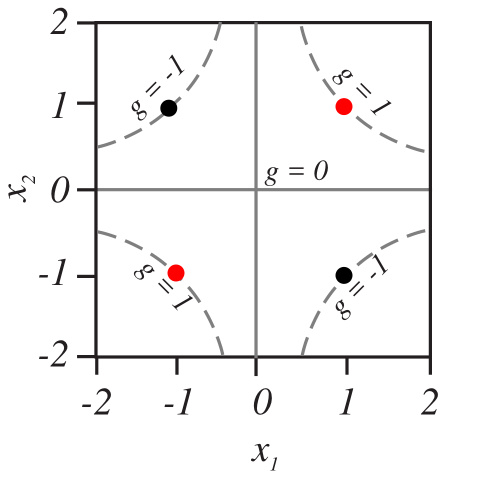
\includegraphics[width=0.3\linewidth]{XOR.PNG}
    \caption{The XOR problem in the original $(x_1,x_2)$ feature space.}
    \label{fig:xor}
\end{figure}

3.1 Consider the polynomial kernel of degree 2: 
\begin{equation}
  K(\bm{x}_i,\bm{x}_j) = (\bm{x_i}^{\top}\bm{x_j}+1)^2,
\end{equation}
where $\bm{x}_i = (x_{i1}, x_{i2})^{\top}$ and $\bm{x}_j=(x_{j1}, x_{j2})^{\top}$.

Show that it corresponds to mapping 
\begin{equation}
  \Phi(x_1, x_2) = \Big[1, \sqrt{2}x_1, \sqrt{2}x_2, \sqrt{2}x_1x_2, x_1^2, x_2^2\Big].
\end{equation}

解: 对核函数有
\begin{equation}
  \begin{aligned}
    K(\bm{x}_i,\bm{x}_j)
      &=(\bm{x_i}^{\top}\bm{x_j}+1)^2\\
      &=(x_{i1}x_{j1}+x_{i2}x_{j2}+1)^2\\
      &=1+x_{i1}^2x_{j1}^2+x_{i2}^2x_{j2}^2+2x_{i1}x_{j1}+2x_{i2}x_{j2}+2x_{i1}x_{j1}x_{i2}x_{j2}\\
  \end{aligned}
\end{equation}

又映射的内积为
\begin{equation}
  \Phi(x_{i1},x_{i2})\cdot\Phi(x_{j1},x_{j2})
  =1+2x_{i1}x_{j1}+2x_{i2}x_{j2}+2x_{i1}x_{j1}x_{i2}x_{j2}+x_{i1}^2x_{j1}^2+x_{i2}^2x_{j2}^2
\end{equation}

则
\begin{equation}
  K(\bm{x}_i,\bm{x}_j)=\Phi(x_{i1},x_{i2})\cdot\Phi(x_{j1},x_{j2})
\end{equation}

因此核函数对应的映射为 $\Phi(\cdot)$.

3.2 Derive the dual problem in the 6-dimensional space with Lagrange multipliers $\alpha_i$, $i=1,2,3,4$ as the only variants.

解: 记 $y_1=1$, $y_2=-1$, $y_3=1$, $y_4=-1$, 
\begin{equation}
  \vx_1=
  \begin{bmatrix}
    1\\ 1\\
  \end{bmatrix},\quad
  \vx_2=
  \begin{bmatrix}
    1\\ -1\\
  \end{bmatrix},\quad
  \vx_3=
  \begin{bmatrix}
    -1\\ -1\\
  \end{bmatrix},\quad
  \vx_4=
  \begin{bmatrix}
    -1\\ 1\\
  \end{bmatrix}
\end{equation}

则原问题为
\begin{equation}
  \begin{aligned}
    &\min_{\vomega}~\frac{1}{2}\|\vomega\|_2^2 \\
    &~\mathrm{s.t.}~~~y_i[\vomega^{\top}\Phi(\vx_i)-b]-1\gs0,~i=1,2,3,4
  \end{aligned}
\end{equation}

引入对偶变量 $\valpha$, 则 Lagrange 函数为
\begin{equation}
  L(\vomega,b,\valpha)=\frac{1}{2}\|\vomega\|_2^2-\sum_{i=1}^4\alpha_i[y_i\vomega^{\top}\Phi(\vx_i)-y_ib-1]
\end{equation}

其对 $\vomega$ 的偏导数为
\begin{equation}
  \frac{\partial L(\vomega,b,\valpha)}{\partial\vomega}=\vomega-\sum_{i=1}^4\alpha_iy_i\Phi(\vx_i)
\end{equation}

令此偏导数为 0, 可得
\begin{equation}
  \vomega=\sum_{i=1}^4\alpha_iy_i\Phi(\vx_i)
\end{equation}

Lagrange 函数对 $b$ 的偏导数为
\begin{equation}
  \frac{\partial L(\vomega,b,\valpha)}{\partial b}=\sum_{i=1}^4\alpha_iy_i
\end{equation}

令此偏导数为 0, 可得
\begin{equation}
  \sum_{i=1}^4\alpha_iy_i=0
\end{equation}

将 $\vomega$ 代入 Lagrange 函数, 可得对偶函数为
\begin{equation}
  Q(\valpha)=-\frac{1}{2}\sum_{i=1}^4\sum_{j=1}^4\alpha_i\alpha_jy_iy_j\Phi(\vx_i)\cdot\Phi(\vx_j)+\sum_{i=1}^4\alpha_i
\end{equation}

所以, 对偶问题为
\begin{equation}
  \begin{aligned}
    &\max_{\valpha}~Q(\valpha)=-\frac{1}{2}\sum_{i=1}^4\sum_{j=1}^4\alpha_i\alpha_jy_iy_j\Phi(\vx_i)\cdot\Phi(\vx_j)+\sum_{i=1}^4\alpha_i\\
    &~\mathrm{s.t.}\quad\sum_{i=1}^4\alpha_iy_i=0\\
    &\quad\quad~~~\alpha_i\gs0,~i=1,2,3,4
  \end{aligned}
\end{equation}

3.3 Solve the dual problem analytically (without programming). What are the support vectors? Hint: use the symmetry of the problem.

解: 对偶函数为
\begin{equation}
  \begin{aligned}
    Q(\valpha)
    &=-\frac{1}{2}\sum_{i=1}^4\sum_{j=1}^4\alpha_i\alpha_jy_iy_j\Phi(\vx_i)\cdot\Phi(\vx_j)+\sum_{i=1}^4\alpha_i\\
    &=\sum_{i=1}^4\alpha_i-\frac{1}{2}\sum_{i=1}^4\sum_{j=1}^4\alpha_i\alpha_jy_iy_jK(\vx_i,\vx_j)\\
  \end{aligned}
\end{equation}

其中 $\forall~i,j=1,2,3,4$, 核函数
\begin{equation}
  K(\vx_i,\vx_j)=
  \begin{cases}
    9,&\text{if}~i=j\\
    1,&\text{otherwise}
  \end{cases}
\end{equation}

则对偶函数对 $\alpha_i$ 的偏导为
\begin{equation}
  \begin{aligned}
    \frac{\partial Q(\valpha)}{\partial\alpha_i}
    &=1-\alpha_iy_iy_iK(\vx_i,\vx_i)-\sum_{j\neq i}\alpha_jy_iy_jK(\vx_i,\vx_j)\\
    &=1-9\alpha_i-y_i\sum_{j\neq i}\alpha_jy_j,\quad\forall~i=1,2,3,4
  \end{aligned}
\end{equation}

又由对偶问题约束可知
\begin{equation}
  \sum_{j\neq i}\alpha_jy_j=\sum_{j=1}^4\alpha_jy_j-\alpha_iy_i=-\alpha_iy_i,\quad\forall~i=1,2,3,4
\end{equation}

代入偏导数表达式可得
\begin{equation}
  \frac{\partial Q(\valpha)}{\partial\alpha_i}
  =1-9\alpha_i+\alpha_iy_iy_i=1-8\alpha_i,\quad\forall~i=1,2,3,4
\end{equation}

令这些偏导数为 0, 有
\begin{equation}
  \alpha_i=\frac{1}{8},\quad\forall~i=1,2,3,4
\end{equation}

则由互补松弛 (complementary slackness) 性可知, $\vx_i$, $i=1,2,3,4$ 都是支持向量.

3.4 Derive the final discriminant function $g(\bm{x})$ and the decision hyperplane.

解: 由上题可知
\begin{equation}
  \begin{aligned}
    \vomega
    &=\sum_{i=1}^4\alpha_iy_i\Phi(\vx_i)\\
    &=\frac{1}{8}
    \left[
      \begin{pmatrix}
        1 \\ \sqrt{2} \\ \sqrt{2} \\ \sqrt{2} \\ 1 \\ 1 \\
      \end{pmatrix}
      -\begin{pmatrix}
        1 \\ \sqrt{2} \\ -\sqrt{2} \\ -\sqrt{2} \\ 1 \\ 1 \\
      \end{pmatrix}
      +\begin{pmatrix}
        1 \\ -\sqrt{2} \\ -\sqrt{2} \\ \sqrt{2} \\ 1 \\ 1 \\
      \end{pmatrix}
      -\begin{pmatrix}
        1 \\ -\sqrt{2} \\ \sqrt{2} \\ -\sqrt{2} \\ 1 \\ 1 \\
      \end{pmatrix}
    \right]\\
    &=\frac{1}{8}
      \begin{pmatrix}
        0 \\ 0 \\ 0 \\ 4\sqrt{2} \\ 0 \\ 0 \\
      \end{pmatrix}
    =\begin{pmatrix}
      0 \\ 0 \\ 0 \\ \frac{\sqrt{2}}{2} \\ 0 \\ 0 \\
    \end{pmatrix}
  \end{aligned}
\end{equation}

所以
\begin{equation}
  \begin{aligned}
    g(\vx)
    &=\vomega^{\top}\Phi(\vx)-b\\
    &=x_1x_2-b\\
  \end{aligned}
\end{equation}

又 $\vx_i$, $i=1,2,3,4$ 都是支持向量, 则有
\begin{equation}
  y_ig(\vx_i)-1=0,\quad\forall~i=1,2,3,4
\end{equation}

从而解得
\begin{equation}
  b=0
\end{equation}

因此, 判别函数为
\begin{equation}
  g(\vx)=x_1x_2
\end{equation}

决策超平面为
\begin{equation}
  g(\vx)=x_1x_2=0
\end{equation}

3.5 Plot the data points on the subspace of $(\sqrt{2}x_1, \sqrt{2}x_1x_2)$. Demonstrate the decision hyperplane and the margin in your plot.

解: 映射到子空间 $(\sqrt{2}x_1, \sqrt{2}x_1x_2)$ 的四个数据点, 决策超平面以及间隔如图 \ref{fig:subxor} 所示.

\begin{figure}[htbp]
  \centering
  \begin{tikzpicture}
    \draw[-latex] (-6,0) -- (6,0) node[below] {$\sqrt{2}x_1$};
    \draw[-latex] (0,-4) -- (0,4) node[left] {$\sqrt{2}x_1x_2$};
    \draw (0,0) node[below left] {0};
    \draw (3,0) node[below right] {$\sqrt{2}$};
    \draw (-3,0) node[below left] {$-\sqrt{2}$};
    \draw (0,3) node[below left] {$\sqrt{2}$};
    \draw (0,-3) node[below left] {$-\sqrt{2}$};
    \draw[dashed] (-3,3) -- (-3,-3);
    \draw[dashed] (3,3) -- (3,-3);
    \draw[dashed,blue] (-4,3) -- (4,3);
    \draw[dashed,blue] (-4,-3) -- (4,-3);
    \draw[line width=1pt,red] (-5.5,0) -- (5.5,0);
    \draw[red] (3.5,0.2) node[above right] {decision hyperplane};
    \fill[red] (3,3) circle (2pt) node[below right] {$\vx_1$};
    \fill[red] (-3,3) circle (2pt) node[below right] {$\vx_3$};
    \fill (-3,-3) circle (2pt) node[below right] {$\vx_4$};
    \fill (3,-3) circle (2pt) node[below right] {$\vx_2$};
    \draw[latex-latex,blue,line width=1pt] (1,3) -- (1,-3);
    \draw[blue] (1,2) node[right] {margin};
  \end{tikzpicture}
  \caption{XOR 问题映射到子空间 $(\sqrt{2}x_1, \sqrt{2}x_1x_2)$, 决策超平面以及间隔}
  \label{fig:subxor}
\end{figure}

\section*{Problem 4}

Write a program to complete the following task adopting the SVM algorithm (you could use some toolkits or source code). Train a SVM classifier with data from $\omega_1$ and $\omega_2$ in the following table. Preprocess each training pattern to form a new vector having components $1,x_1,x_2,x_1^2,x_1x_2$ and $ x_2^2$.

\begin{table}[ht]
	\centering
	\begin{tabular}{ccccc}
		\hline
    ~&\multicolumn{2}{c}{$\omega_1$} & \multicolumn{2}{c}{$\omega_2$}\\
    \cmidrule(r){2-3} \cmidrule(r){4-5}
		sample & $x_1$ & $x_2$ & $x_1$ & $x_2$\\
		\hline
		1  & -3.0 & -2.9 & -2.0 & -8.4\\
		2  & 0.5  & 8.7 & -8.9 & 0.2\\
		3  & 2.9  & 2.1 & -4.2 & -7.7\\
		4  & -0.1 & 5.2 & -8.5 & -3.2\\
		5  & -4.0 & 2.2 & -6.7 & -4.0\\
		6  & -1.3 & 3.7 & -0.5 & -9.2\\
		7  & -3.4 & 6.2 & -5.3 & -6.7\\
		8  & -4.1 & 3.4 & -8.7 & -6.4\\
		9  & -5.1 & 1.6 & -7.1 & -9.7\\
		10 & 1.9  & 5.1 & -8.0 & -6.3\\
		\hline
	\end{tabular}
\end{table}

Hint: You needn't program the SVM algorithm by yourself, you can just use some toolkits or source code such as \href{http://www.csie.ntu.edu.tw/~cjlin/libsvm/}{libsvm} for MATLAB or \href{https://scikit-learn.org/stable/modules/svm.html#svm-classification}{scikit-learn} for python. You should declare the toolkit you used in your project.

4.1 Train you classifier with just the first point in the $\omega_1$ and $\omega_2$ and find the separating hyperplane and the margin.

解: 使用 MATLAB 内置 \verb|fitcsvm| 函数, 对两个类别的第一个点训练 SVM 得到分类边界如图 \ref{fig:svm1} 中蓝色实线所示, 分类超平面的表达式为
\begin{equation}
  g(\vx)=w_1+w_2x_1+w_3x_2+w_4x_1^2+w_5x_1x_2+w_6x_2^2+b=0
\end{equation}

其中 $w_i$, $i=1,2,\dots,6$ 的数值见表 \ref{tab:svm} 中第一行, 且间隔 (margin) 为
\begin{equation}
  \mathrm{margin}=63.1228
\end{equation}

\begin{figure}[htbp]
  \centering
  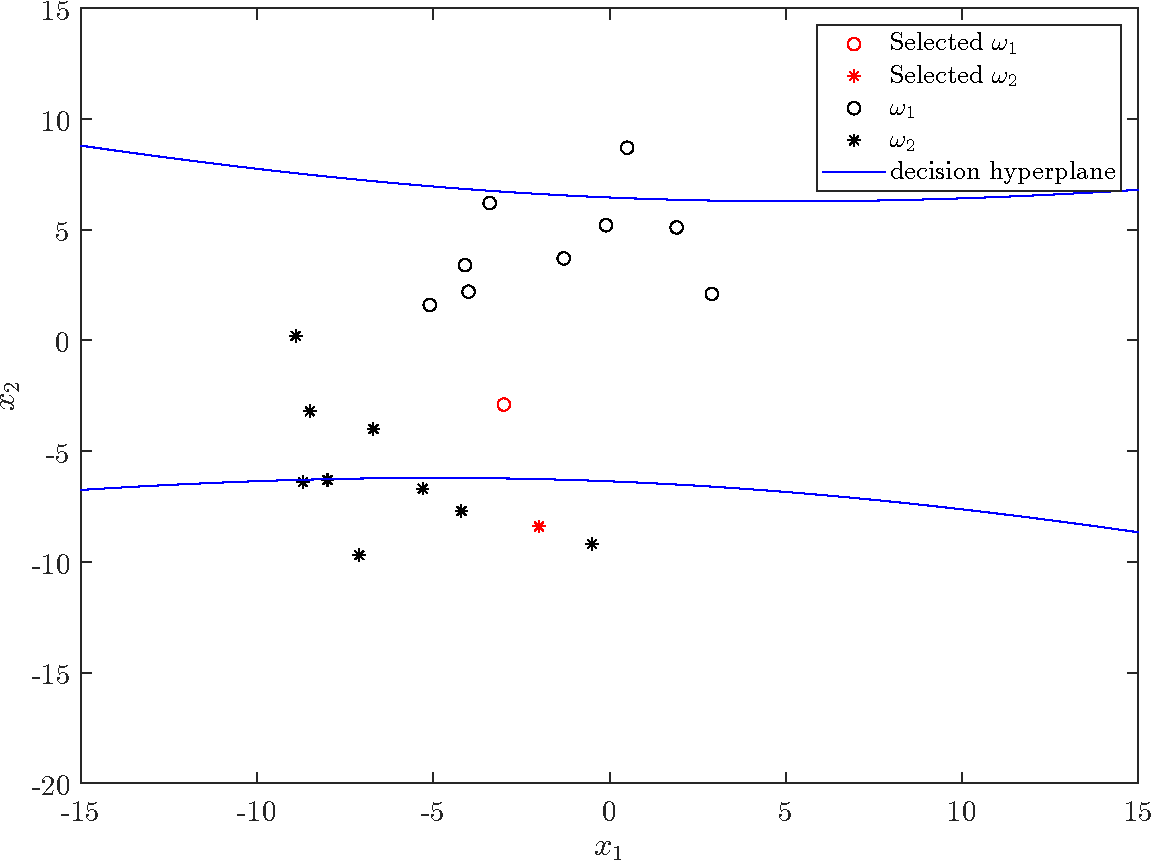
\includegraphics[width=16cm]{svmPoint1.pdf}
  \caption{使用两类第一个点训练 SVM 得到分类边界}
  \label{fig:svm1}
\end{figure}

\begin{table}[htbp]
  \centering
  \caption{分别使用前 1 至 10 个点训练 SVM 得到分类超平面参数和间隔}
  \label{tab:svm}
  \begin{tabular}{ccccccccc}
    \hline
    \# of Points & $w_1$ & $w_2$   & $w_3$  & $w_4$   & $w_5$   & $w_6$   & $b$    & margin  \\
    \hline
    1   & 0     & -0.0005 & 0.0028 & 0.0025  & -0.0041 & -0.0312 & 1.2816 & 63.1228 \\
    2   & 0     & 0.0121  & 0.0739 & -0.0413 & -0.0534 & -0.0222 & 2.2739 & 19.3674 \\
    3   & 0     & 0.0121  & 0.0739 & -0.0413 & -0.0534 & -0.0222 & 2.2739 & 19.3674 \\
    4   & 0     & 0.0121  & 0.0739 & -0.0413 & -0.0534 & -0.0222 & 2.2739 & 19.3674 \\
    5   & 0     & 0.0121  & 0.0739 & -0.0413 & -0.0534 & -0.0222 & 2.2740 & 19.3686 \\
    6   & 0     & 0.0111  & 0.0989 & -0.0379 & -0.0210 & -0.0239 & 2.0453 & 17.9957 \\
    7   & 0     & 0.0111  & 0.0989 & -0.0379 & -0.0210 & -0.0239 & 2.0453 & 17.9957 \\
    8   & 0     & 0.0111  & 0.0989 & -0.0379 & -0.0210 & -0.0239 & 2.0453 & 17.9957 \\
    9   & 0     & 0.0111  & 0.0989 & -0.0379 & -0.0210 & -0.0239 & 2.0451 & 17.9976 \\
    10  & 0     & 0.0111  & 0.0989 & -0.0379 & -0.0210 & -0.0239 & 2.0451 & 17.9976\\
    \hline
  \end{tabular}
\end{table}

4.2 Repeat 4.1 with the first two points in each category (four points total), the first three points and so on, until the transformed patterns cannot be linearly separated in the transformed space.

解: 依次使用前 2 至前 10 个点训练 SVM 得到分类边界如图 \ref{fig:svm2} 所示, 分类超平面的参数以及间隔如表 \ref{tab:svm} 所示. 由图可知依次生成的训练集数据在转换后的空间上均是线性可分的, 随着训练点数的增多, 间隔逐渐减小, 但是如果新增的点不是支持向量, 则对分类面没有影响.

\begin{figure}[htbp]
  \centering
  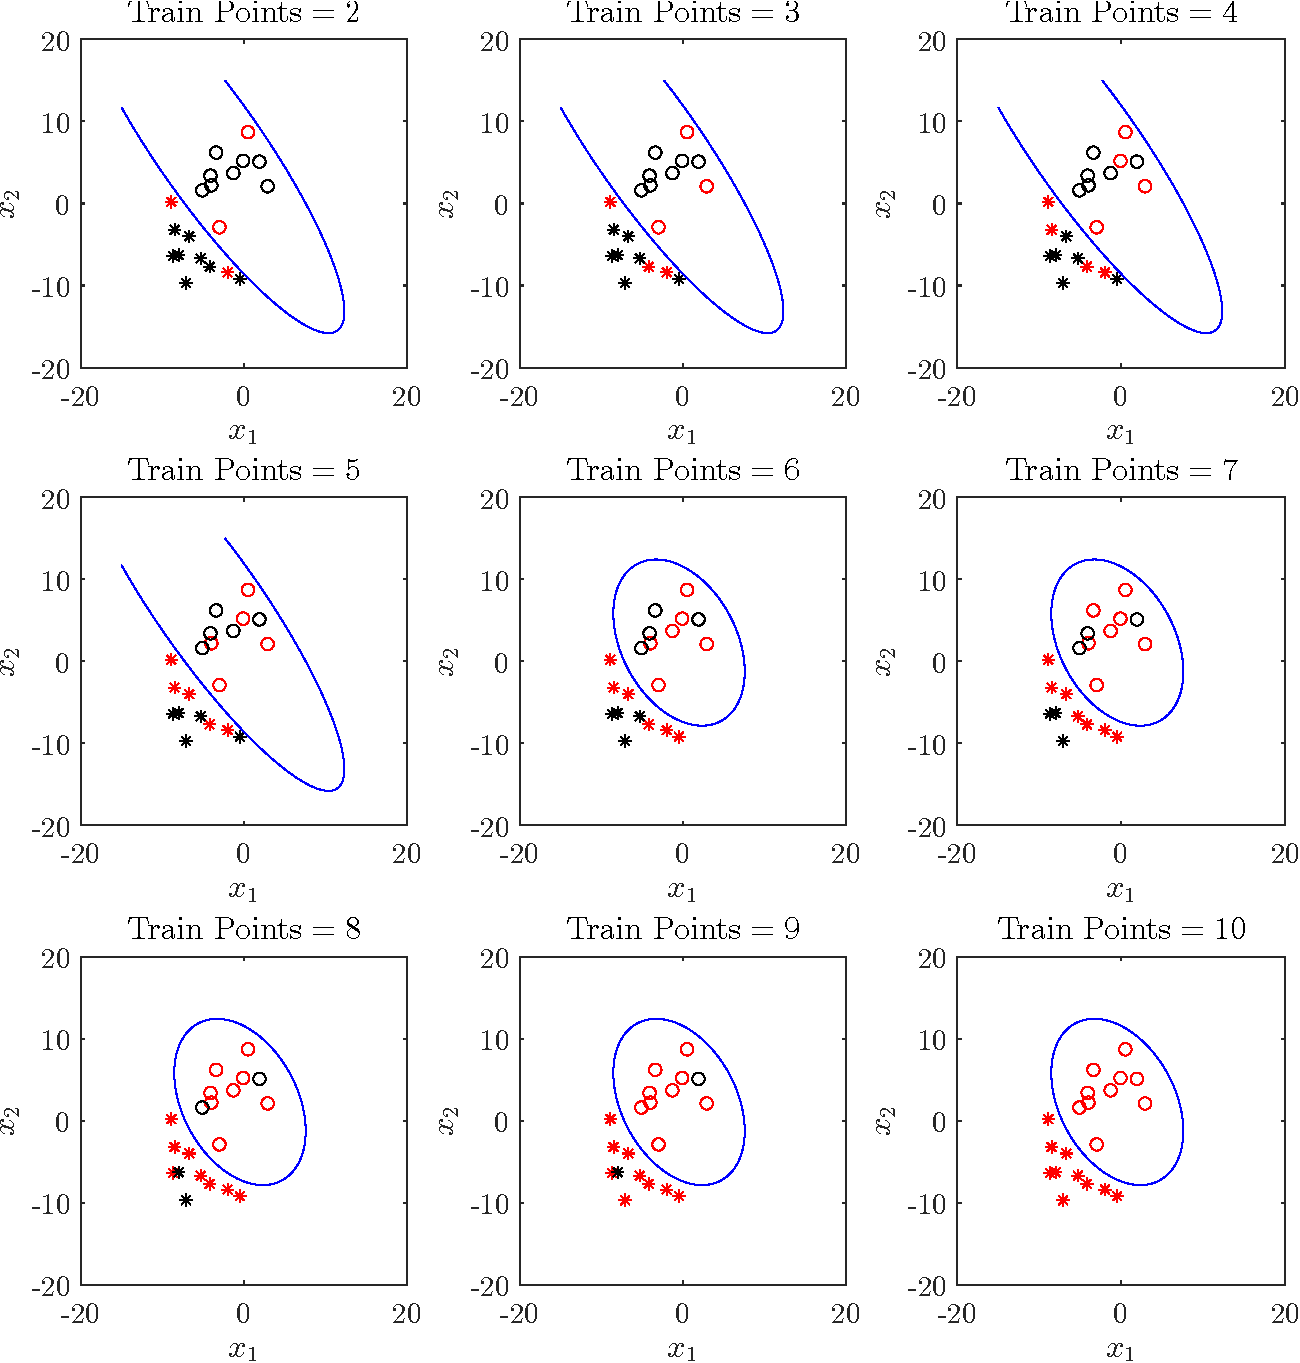
\includegraphics[width=16cm]{svmPoint2-10.pdf}
  \caption{依次使用前 2 至前 10 个点训练 SVM 得到分类边界}
  \label{fig:svm2}
\end{figure}

% Reference
% \begin{thebibliography}{1}
%   \bibitem{b1}{Flying pig. Deriving the conditional distributions of a multivariate normal distribution, 2012. \href{https://stats.stackexchange.com/questions/30588}{https://stats.stackexchange.com/questions/30588}}
% \end{thebibliography}

\end{document}
